\RequirePackage{flashmovie/flashmovie}

\documentclass[10pt,colorlinks]{beamer}
  % compress
  %\documentclass[handout,xcolot=pdftex,dvipsnames,table]{beamer}

\definecolor{mybg}{RGB}{255,255,204}
\usepackage{minted}
\usepackage{graphicx}
\usepackage[english]{babel}
\usepackage[utf8x]{inputenc}
\usepackage{amsmath}
\usepackage{longtable}
% \usepackage[table]{xcolor}
 \usepackage{beamerthemesplit}

%\usemintedstyle{trac}

\mode<presentation>
\setbeamercovered{invisible}
\usetheme{Warsaw}
\usecolortheme{dolphin}

\usefonttheme{serif}







% Delete this, if you do not want the table of contents to pop up at
% the beginning of each subsection:
\AtBeginSection[]
{
  \begin{frame}<beamer,allowframebreaks>{Outline}
    \tableofcontents[currentsection]
  \end{frame}
}



\title{ Python para RPi}
\subtitle
{Parte III: Introduction a la Raspberry PI} % (optional)


\author[Velasco and Perera]{Manel Velasco,\inst{1} PhD and Alexandre Perera,\inst{1}$^{,}$\inst{2} PhD}

\institute[UPC] % (optional, but mostly needed)
{
  \inst{1}%
  Departament d'Enginyeria de Sistemes, Automatica i Informatica Industrial (ESAII)  \\
  Universitat Politecnica de Catalunya 
  \and 
  \inst{2}%
   Centro de Investigacion Biomedica en Red en Bioingenieria, Biomateriales y Nanomedicina (CIBER-BBN)  \\
    \href{mailto:Alexandre.Perera@upc.edu}{Alexandre.Perera@upc.edu}~\href{mailto:manel.velasco@upc.edu}{Manel.Velasco@upc.edu}
}
 

\date[Feb, 2013, Learning Python]{Introduction to Python for Engineering and Statistics\\
Febraury, 2013}

 %

\begin{document}


\begin{frame}[plain]
   %  \titlepage
   \maketitle
\end{frame}


\begin{frame}[allowframebreaks]{Contents}
  \tableofcontents
  % You might wish to add the option [pausesections]
 \note[options]{aixo son notes}
\end{frame}

\section{Introduction}
\subsection{Raspberry Pi Foundation}
%----------------------------FRAME 2 cols------------------------------
\begin{frame}[fragile]\frametitle{Raspberry Pi}
\begin{columns}[c]
\column{0.5\textwidth}
\begin{block}{RPI Foundation}
\begin{itemize}
    \item  La Raspberry Pi Foundation es una organización sin ánimo de lucro establecida  como fundación en 2008.

\item En 2011 desarrolló la Raspberry Pi como ordenador de bajo coste para facilitar la enseñanza de la informática en los colegios.
 
\item Entró en producción el 2012. La fundación recibe apoyos del laboratorio de informática de la Universidad de Cambridge y de Broadcom.
\end{itemize}

\end{block}

\column{0.5\textwidth}
    \centering
    
\includegraphics[width=1\textwidth]{figs/rpi}
\end{columns}
\end{frame}

\section{RPi Board}
\subsection{Especificaciones de la RPi}
%----------------------------FRAME------------------------------------
\begin{frame}[allowframebreaks]\frametitle{Specificaciones}
\small \begin{longtable}[c]{|p{1.3cm}||p{7cm}|p{2.1cm}|} \hline  
& Modelo A & Modelo B
\\  
\hline \hline  
Precio: & \$25 & \$35
\\   \hline

SoC:&\multicolumn{2}{p{9cm}|}{ BCM2835 (CPU + GPU
+  DSP + SDRAM +
USB)}
\\  \hline
 
CPU: & \multicolumn{2}{p{9cm}|}{ ARM1176JZF-Sx a 700~MHz (familia
ARM11)}
\\ \hline
  
GPU: & \multicolumn{2}{p{9cm}|}{ BCM VideoCore IV, , OpenGL ES 2.0, -2 y
VC-1 (con licencia), 1080p30
H.264/MPEG-4 AVC}
\\ \hline
  
Mem.: & 256 MB (comp. GPU) & 512 MB
15/10/2012
\\ \hline
  
 
Ent. Víd: & \multicolumn{2}{p{9cm}|}{ Conector MIPI
CSI (RPF webcam)}
\\ \hline
  
Víd.: &  \multicolumn{2}{p{9cm}|}{ RCA  (PAL
y NTSC), HDMI (rev1.3 y 1.4), 
DSI (LCD)}

\\ \hline
  
Audio: & \multicolumn{2}{p{9cm}|}{ Jack  3.5
mm, HDMI}
\\ \hline
  
Almac.: & \multicolumn{2}{p{9cm}|}{ Tarjeta SD /
MultiMediaCard MMC / SDIO}
\\ \hline
  
Red: & Ninguna & 10/100 Ethernet
(RJ-45) via hub USB
\\ \hline
  
Perif.: &\multicolumn{2}{p{9cm}|}{ 
8~x~General Purpose Input/Output GPIO,
Serial Peripheral Interface SPI, Ii$^2$C,
Universal Asynchronous Receiver-Transmitter UART}
\\  \hline
 
RTClk: &\multicolumn{2}{p{9cm}|}{ 
Ninguno}
\\  \hline
 
Cons.: & 500~mA, (2.5 W) & 700~mA, (3.5 W)
\\ \hline
  
Alim.: &\multicolumn{2}{p{9cm}|}{  5~V vía Micro USB o GPIO header}
\\ \hline
  
Dims: &\multicolumn{2}{p{9cm}|}{  85.60mm × 53.98mm (3.370 × 2.125 inch)}
\\ \hline
  
SO: & \multicolumn{2}{p{9cm}|}{ GNU/Linux: Debian
(Raspbian), Fedora (distribución Linux) (Pidora),
Arch Linux (Arch Linux
ARM) , Slackware Linux . RISC OS}
\\  
\hline \hline
\end{longtable}

\end{frame}

%----------------------------FRAME------------------------------------
\begin{frame}[fragile]\frametitle{Raspberry Pi}

    \centering
    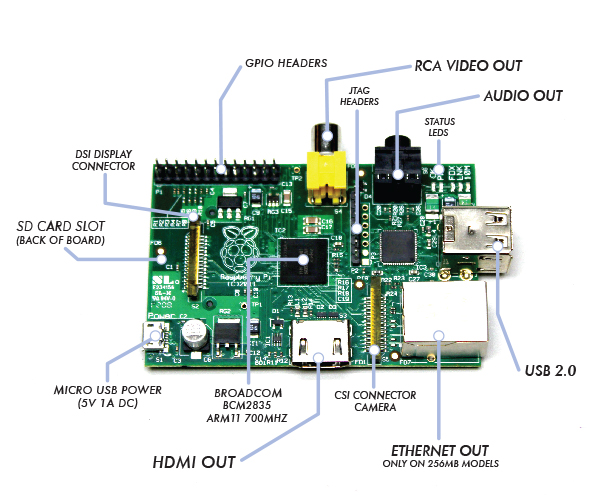
\includegraphics[width=.9\textwidth]{figs/pischeme}

\end{frame}



%----------------------------FRAME 2 cols------------------------------
\begin{frame}[plain]\frametitle{Pinout Rev2 B}
\begin{center}
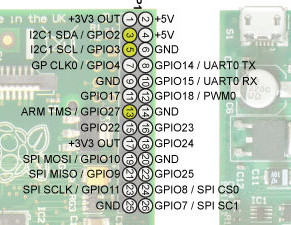
\includegraphics[width=0.9\linewidth]{figs/pinoutsBz}
\end{center}
\end{frame}


%----------------------------FRAME 2 cols------------------------------
\begin{frame}[plain]\frametitle{Pinout Rev2B vs. Rev1B}
\begin{center}
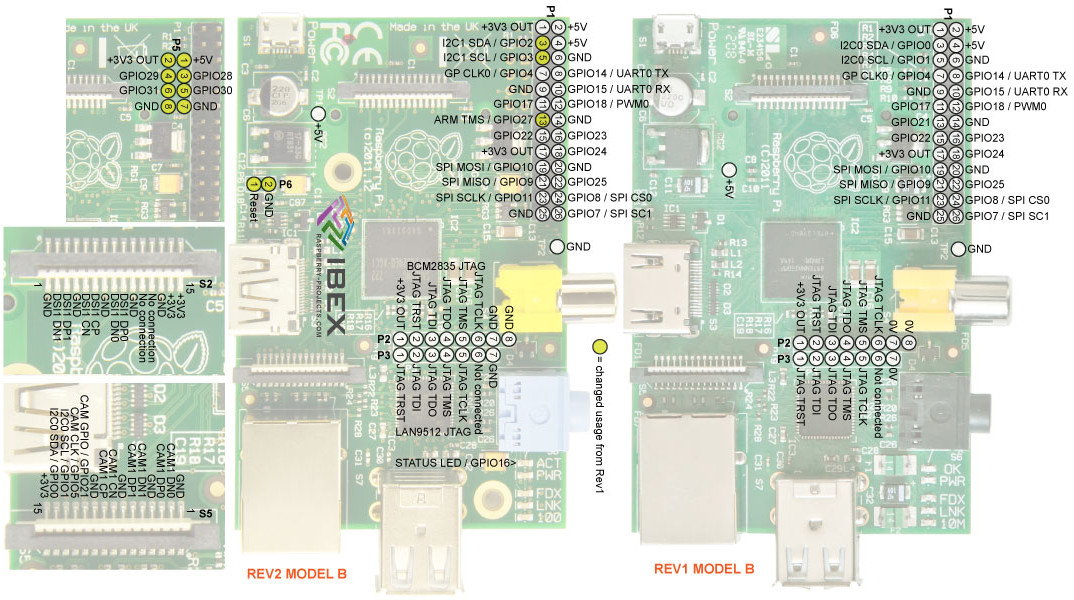
\includegraphics[width=1.1\linewidth]{figs/pinoutsB}
\end{center}
\end{frame}


% Aquest és el pinout de la Rev1 B
%----------------------------FRAME 2 cols------------------------------
%\begin{frame}[plain]\frametitle{Pinout}
%\begin{columns}[c]
%\column{0.5\textwidth}
%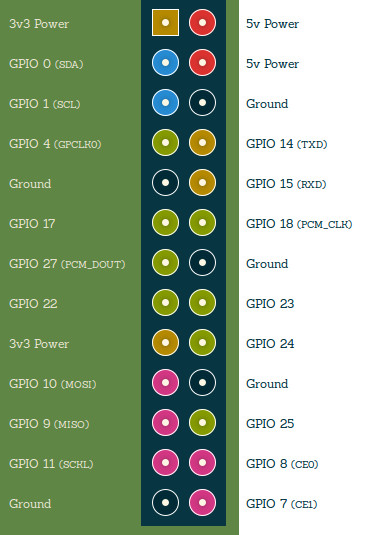
\includegraphics[width=0.5\linewidth]{figs/pinout}
%\column{0.5\textwidth}


%\end{columns}
%\end{frame}


%----------------------------FRAME------------------------------------
\begin{frame}[allowframebreaks]\frametitle{Notas}
\begin{block}{Potencia}
\begin{itemize}
    \item Es necesario un alimentador USB de 700mA a 5V (1A recomendado). 
    \item Cargadores de teléfonos móviles. 
    \item Extremadamente sensible, si la alimentación baja de 5V el comportamiento de la RPi es errático. 
\end{itemize}
\end{block}

\begin{block}{SD Card}
Tamaño mínimo 4Gb de clase 4. El acceso es muuuuuuy lento. factor crítico en el desempeño de todo el sistema. 
\end{block}
\begin{block}{HDMI/Vídeo}
\begin{itemize}
    \item HDMI a HDMI (Incluyendo soporte para audio digital y HDMI-CEC !!).
    \item HDMI a DVI.
    \item Conector estándar RCA de vídeo compuesto.
\end{itemize}
\end{block}


 \begin{center}
    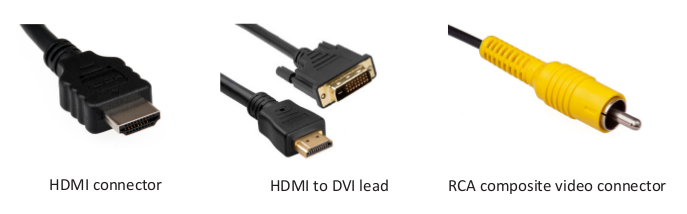
\includegraphics[width=\textwidth]{figs/leads}
\end{center}


\begin{block}{USB}
\begin{itemize}
    \item Cualquier teclado/ratón USB funciona siempre que no requiera mucha potencia al bus USB.
    \item Existen varias Cámaras USB listadas como compatibles (UVC, en general las que tienen soporte GNU/Linux ARM)  
    \item USB hubs, depende de cada caso... 
\end{itemize}
\end{block}

%\begin{block}{Ethernet}
%%Sólo en modelo B
%\end{block}

\end{frame}


\subsection{Accesorios}

%----------------------------FRAME 2 cols------------------------------
\begin{frame}[fragile]\frametitle{Cajas I}
\begin{columns}[c]
 \column{0.5\textwidth}
  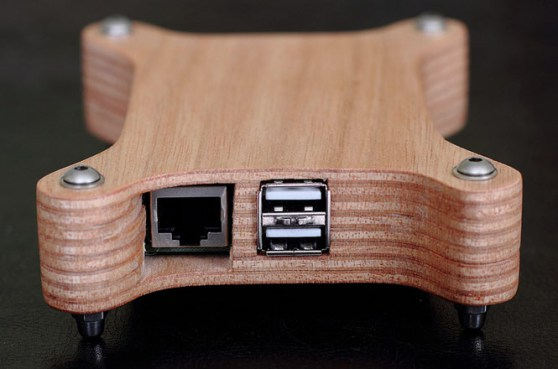
\includegraphics[width=\textwidth]{figs/case3}
 \column{0.5\textwidth}
 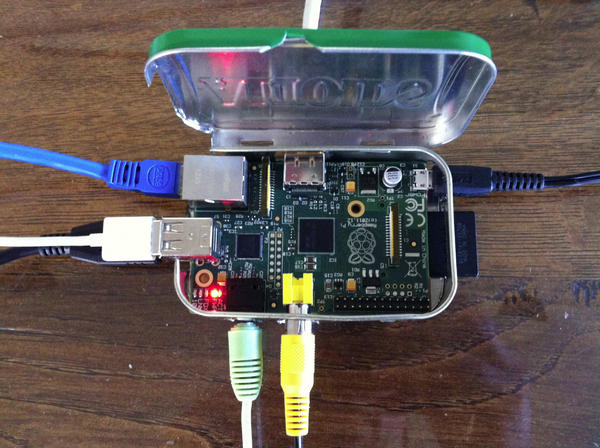
\includegraphics[width=\textwidth]{figs/case4}
 \end{columns}
\end{frame}
 
%----------------------------FRAME 2 cols------------------------------
\begin{frame}[fragile]\frametitle{Cajas II}
\begin{columns}[c]
\column{0.5\textwidth}
 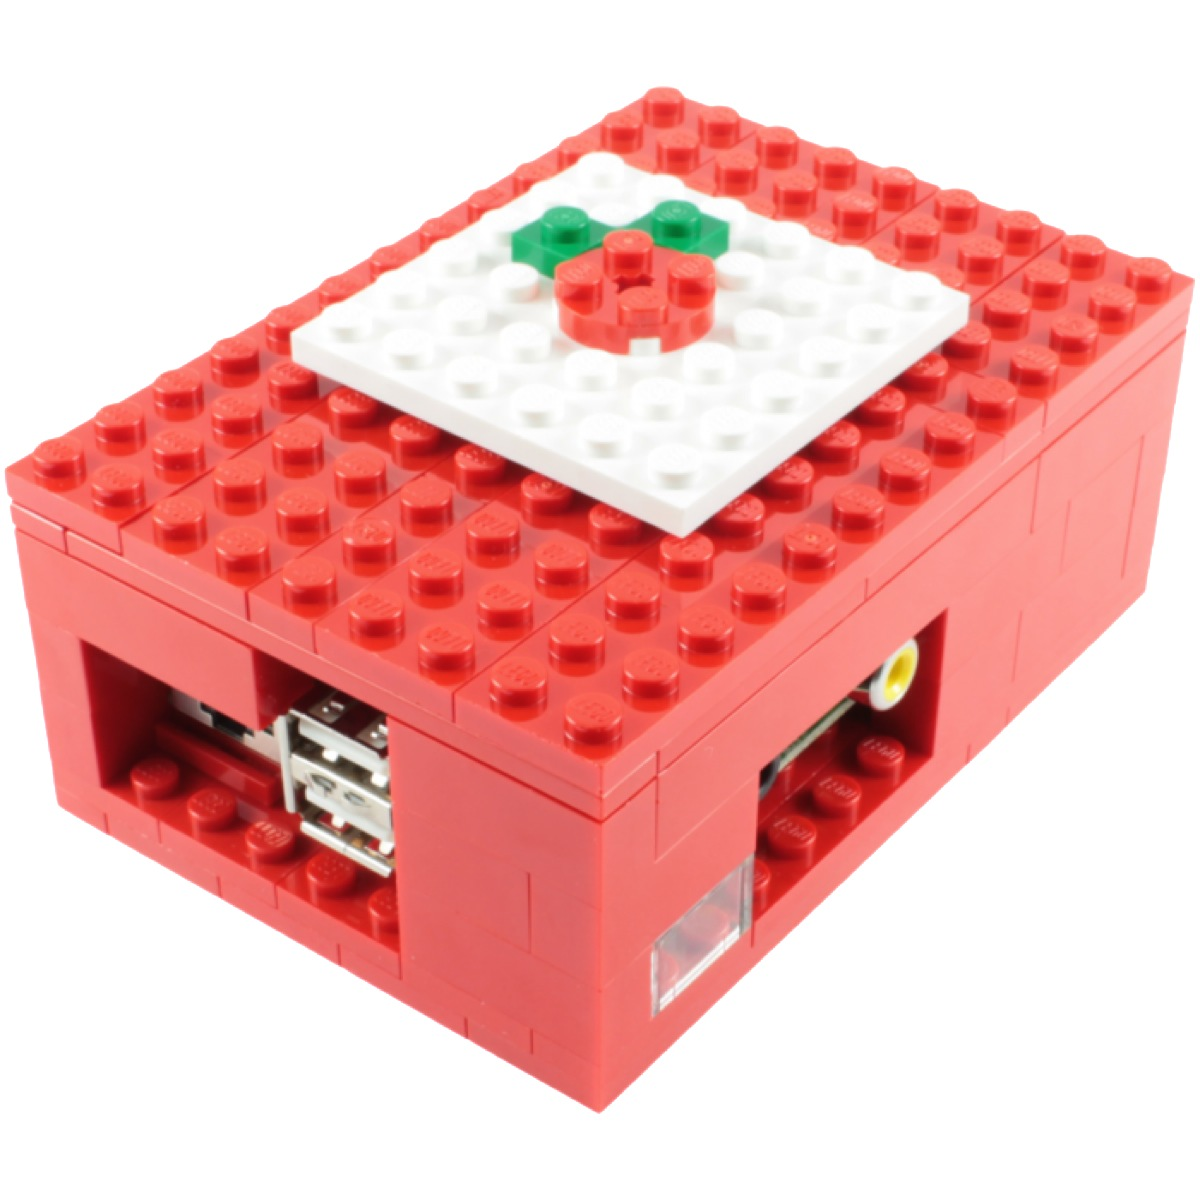
\includegraphics[width=\textwidth]{figs/case1}
\column{0.5\textwidth}
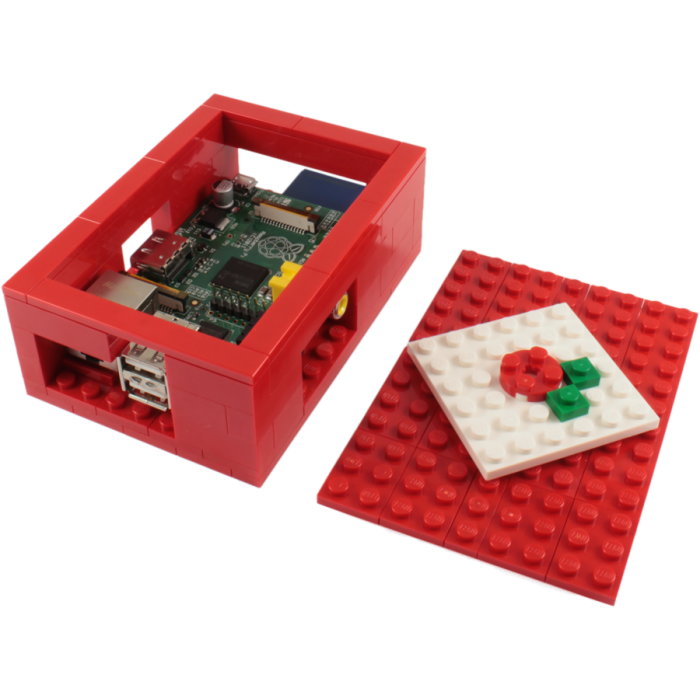
\includegraphics[width=\textwidth]{figs/case2}
\end{columns}
\end{frame}



%----------------------------FRAME 2 cols------------------------------
\begin{frame}\frametitle{Cajas III}

   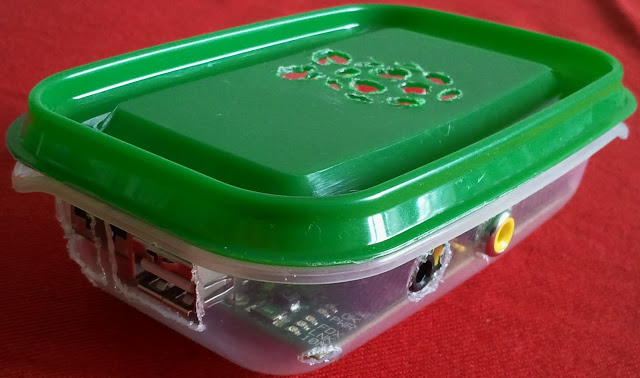
\includegraphics[width=\textwidth]{figs/case5}

\end{frame}
 
\begin{frame}[plain]\frametitle{Element 14}

   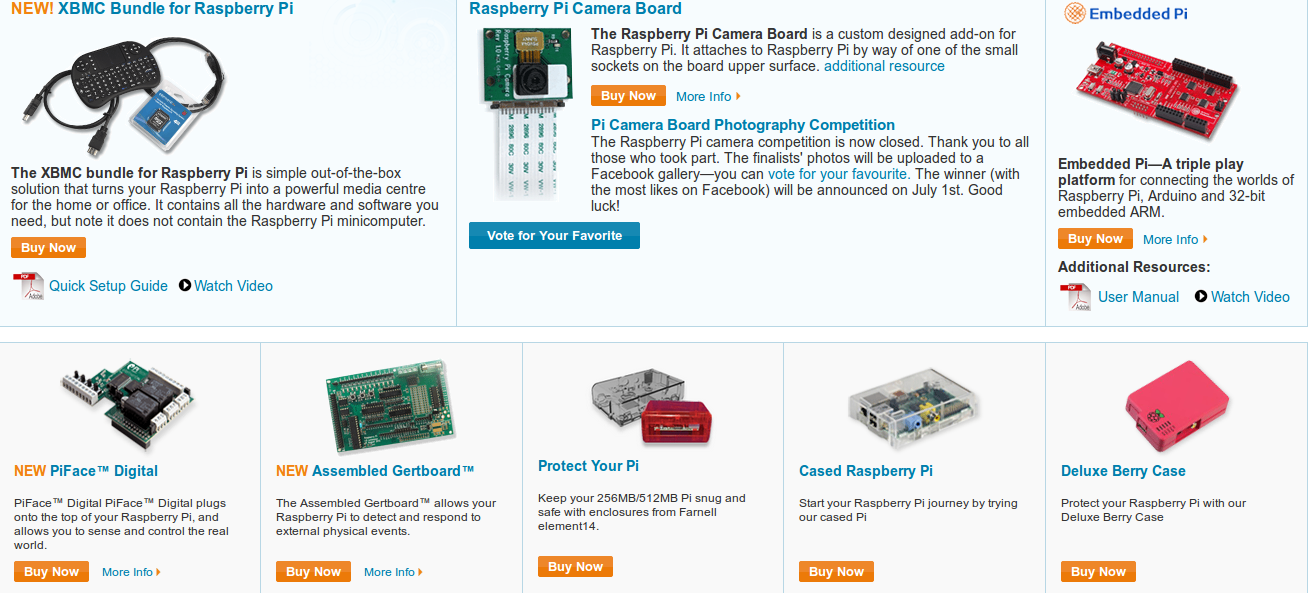
\includegraphics[width=\textwidth]{figs/element}\\
\href{http://www.element14.com/community/groups/raspberry-pi-accessories}{http://www.element14.com/community/groups/raspberry-pi-accessories}
\end{frame}


%----------------------------FRAME------------------------------------
\begin{frame}[fragile]\frametitle{ModMyPi}
   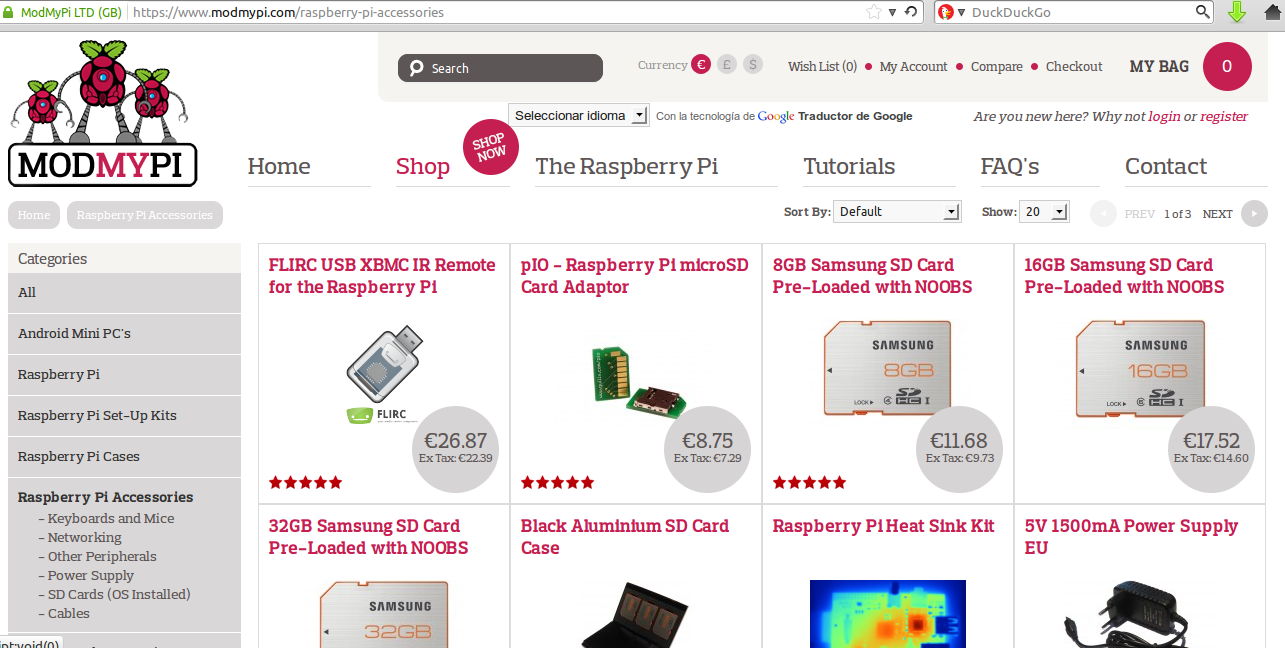
\includegraphics[width=\textwidth]{figs/modmypi}\\
\href{https://www.modmypi.com/raspberry-pi-accessories}{https://www.modmypi.com/raspberry-pi-accessories}

\end{frame}


\subsection{Compatibilidad}                               
%----------------------------FRAME------------------------------------
\begin{frame}\frametitle{Compatibilidad}
    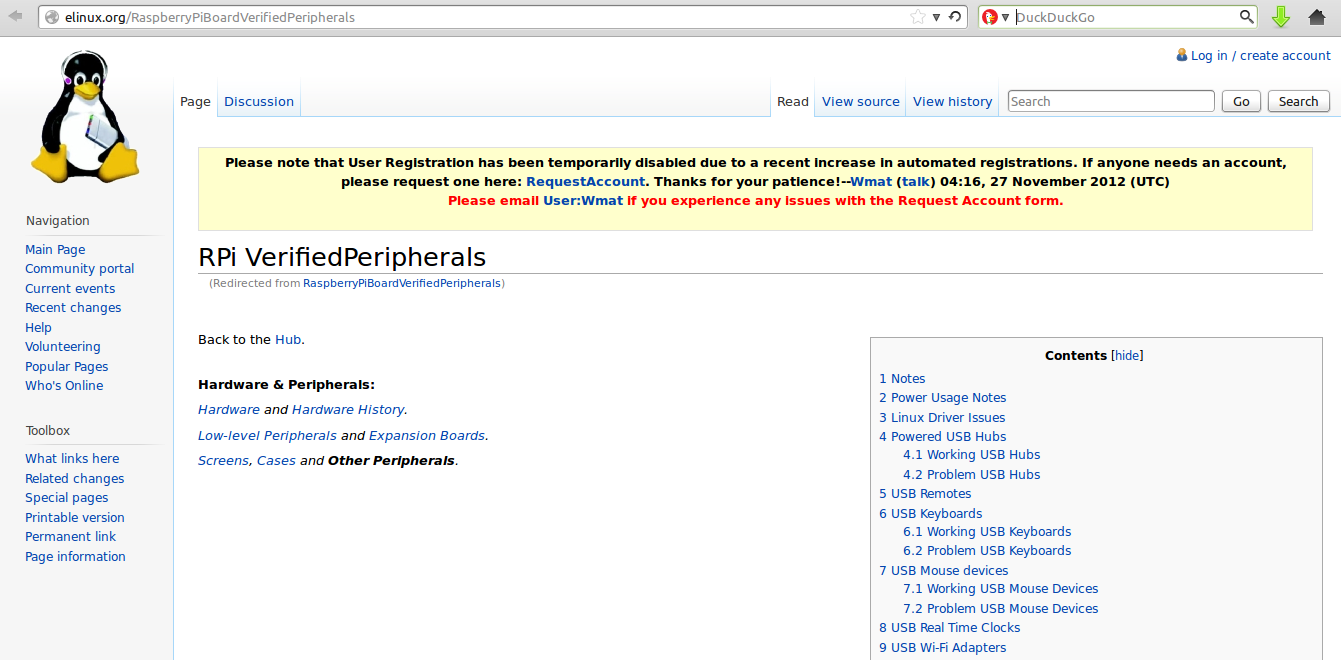
\includegraphics[width=\textwidth]{figs/elinux1}\\
\href{http://elinux.org/RaspberryPiBoardVerifiedPeripherals}{http://elinux.org/RaspberryPiBoardVerifiedPeripherals}
\end{frame}

%----------------------------FRAME------------------------------------
\begin{frame}[plain]\frametitle{Compatibilidad}
    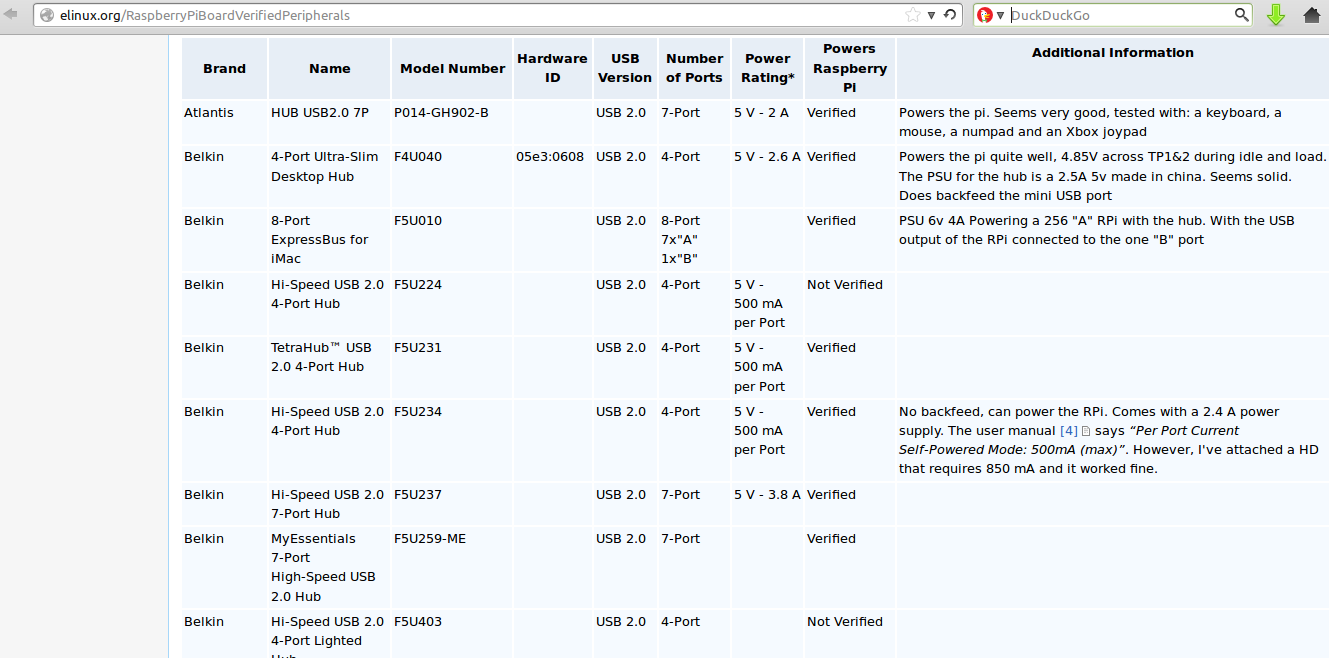
\includegraphics[width=\textwidth]{figs/elinux2}\\
\href{http://elinux.org/RaspberryPiBoardVerifiedPeripherals}{http://elinux.org/RaspberryPiBoardVerifiedPeripherals}
\end{frame}

%----------------------------FRAME------------------------------------
\begin{frame}[plain]\frametitle{Compatibilidad}
    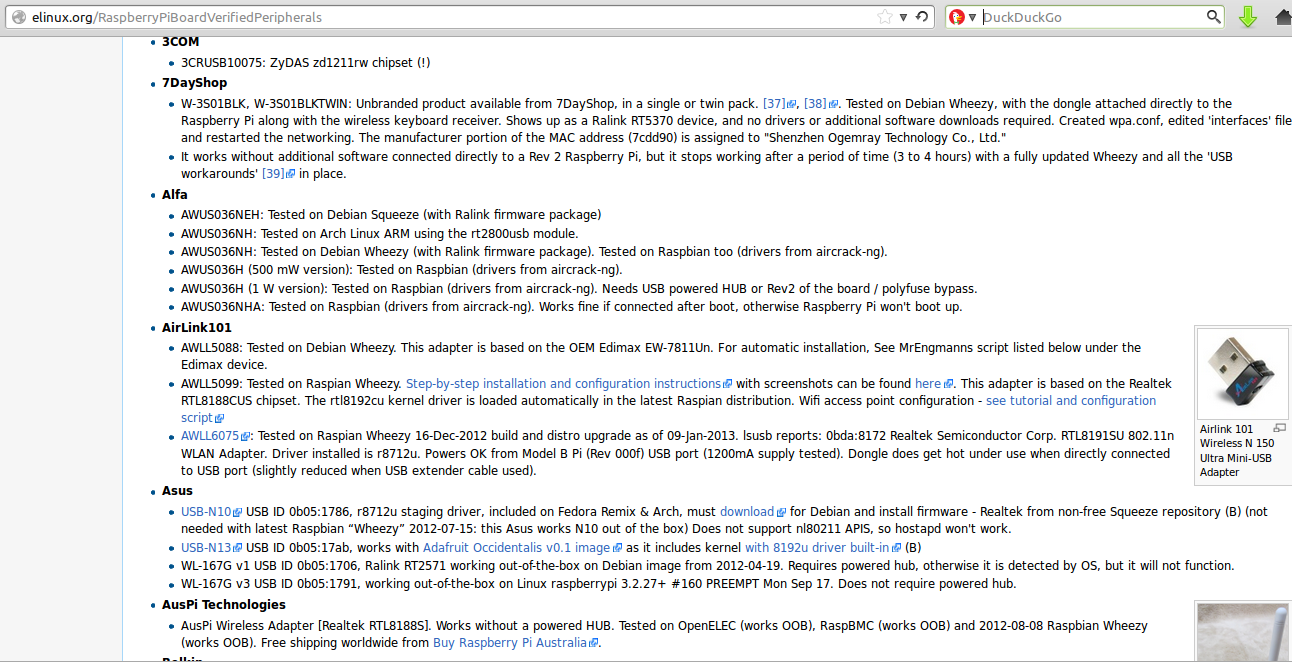
\includegraphics[width=\textwidth]{figs/elinux3}\\
\href{http://elinux.org/RaspberryPiBoardVerifiedPeripherals}{http://elinux.org/RaspberryPiBoardVerifiedPeripherals}
\end{frame}


%----------------------------FRAME------------------------------------
\begin{frame}[plain]\frametitle{Compatibilidad}
    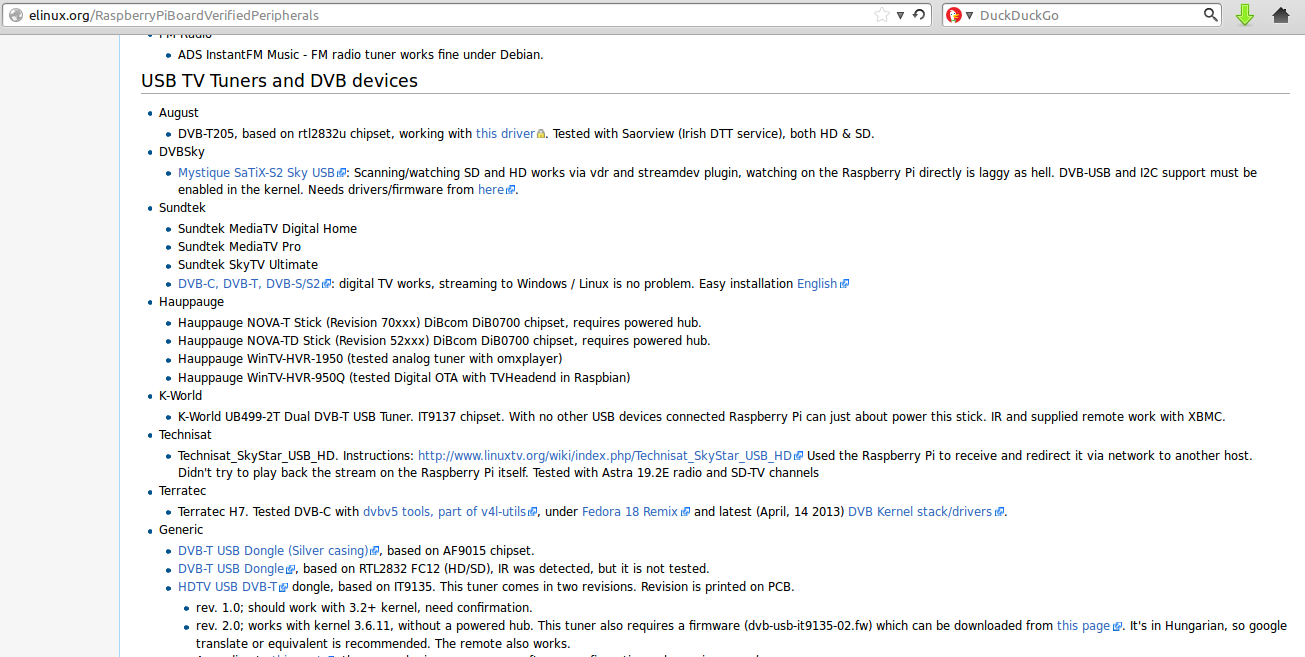
\includegraphics[width=\textwidth]{figs/elinux4}\\
\href{http://elinux.org/RaspberryPiBoardVerifiedPeripherals}{http://elinux.org/RaspberryPiBoardVerifiedPeripherals}
\end{frame}


%----------------------------FRAME------------------------------------
\begin{frame}[plain]\frametitle{Compatibilidad}
    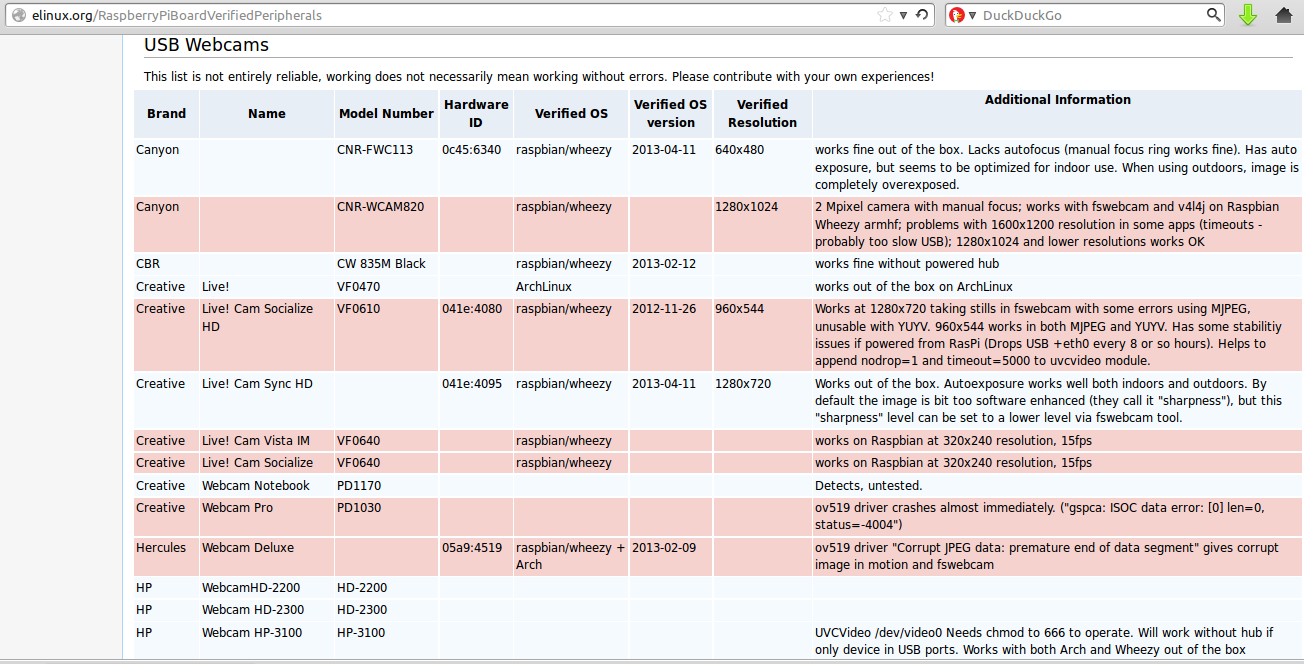
\includegraphics[width=\textwidth]{figs/elinux5}\\
\href{http://elinux.org/RaspberryPiBoardVerifiedPeripherals}{http://elinux.org/RaspberryPiBoardVerifiedPeripherals}
\end{frame}

\section{Instalación}

\subsection{SD}
%----------------------------FRAME------------------------------------
\begin{frame}[allowframebreaks]\frametitle{Preparando una SD para la RPi}
Intrucciones paso a paso.

\begin{block}{Tarjeta SD}
Insertar una tarjeta SD de como mínimo 4Gb.
\end{block}

\begin{block}{Formatear la tarjeta SD}

\begin{description}

    \item[Windows] \href{https://www.sdcard.org/downloads/formatter\_4/eula\_windows/}{https://www.sdcard.org/downloads/formatter\_4/eula\_windows/}, La opción de FORMAT SIZE ADJUSTMENT debe estar en ON. 

    \item[OS X] \href{https://www.sdcard.org/downloads/forma    tter\_4/eula\_mac/}{https://www.sdcard.org/downloads/formatter\_4/eula\_mac/}, Seleccionar la opción "Overwrite Format".

    \item[Linux] Usar \emph{gparted}, formatear como FAT.  

\end{description}

\end{block}



\end{frame}


\subsection{NOOBS}
%----------------------------FRAME------------------------------------
\begin{frame}[fragile]\frametitle{Preparando una SD para la RPi}
\begin{block}{New Out Of the Box Software}

\begin{enumerate}
    \item Descargar NOOBS (ZIP de 1Gb )\\
     \href{downloads.raspberrypi.org/noobs}{downloads.raspberrypi.org/noobs}
    \item Descomprimir el ZIP. 
    \item Copiar el contenido del ZIP en la tarjeta SD. 
    \item Listo!
\end{enumerate}

\end{block}

\begin{block}{NOOBS}
\begin{itemize}
    \item NOOBS crea una Recovery Partition accesible mediante el uso de SHIFT al arrancar. 
    \item Nos permite conmutar SOs o reparar una instalación corrupta.
    \item Contiene un editor de ficheros. 
    \item Contiene un navegador (Arora)
\end{itemize}
\end{block}

\end{frame}


%----------------------------FRAME------------------------------------
\begin{frame}[fragile]\frametitle{NOOBS}
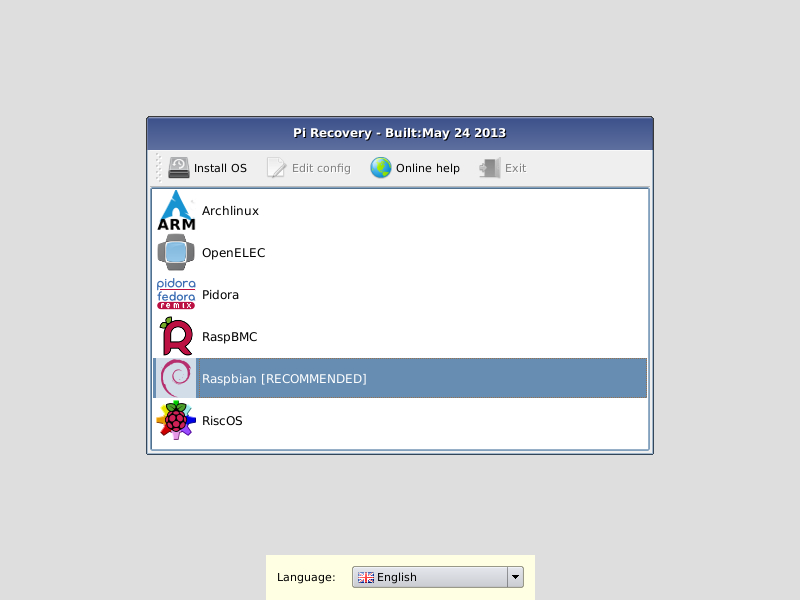
\includegraphics[width=0.8\textwidth]{figs/noobs1}
\end{frame}


%----------------------------FRAME------------------------------------
\begin{frame}[fragile]\frametitle{NOOBS}
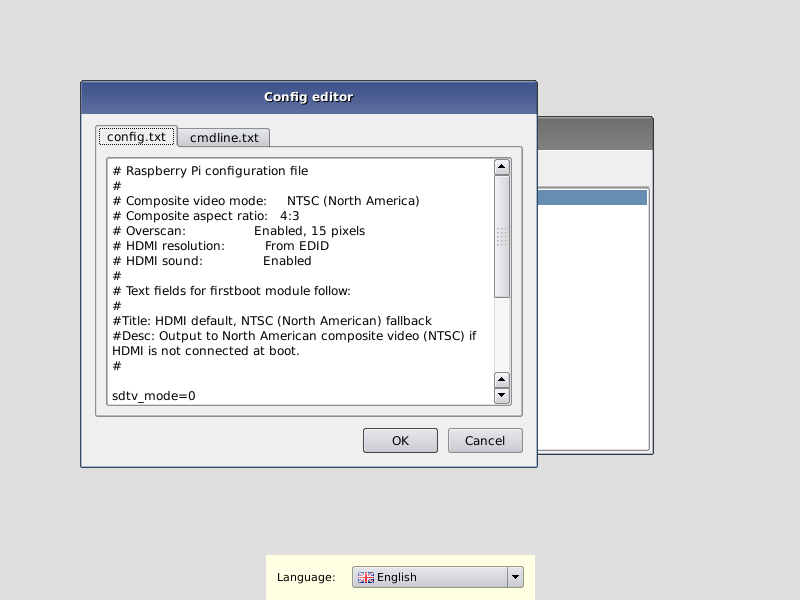
\includegraphics[width=0.8\textwidth]{figs/noobs2}
\end{frame}

%----------------------------FRAME------------------------------------
\begin{frame}[fragile]\frametitle{NOOBS}
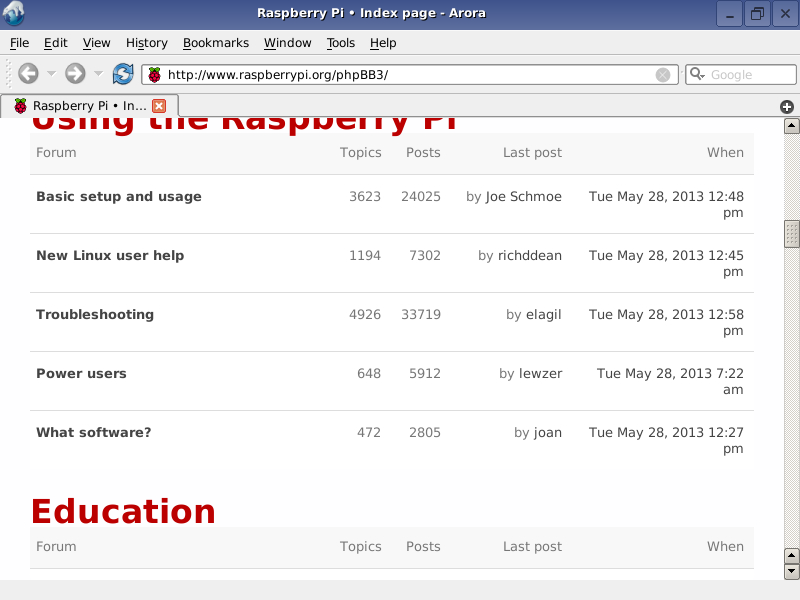
\includegraphics[width=0.8\textwidth]{figs/noobs3}
\end{frame}


%----------------------------FRAME------------------------------------
\begin{frame}[fragile]\frametitle{NOOBS}
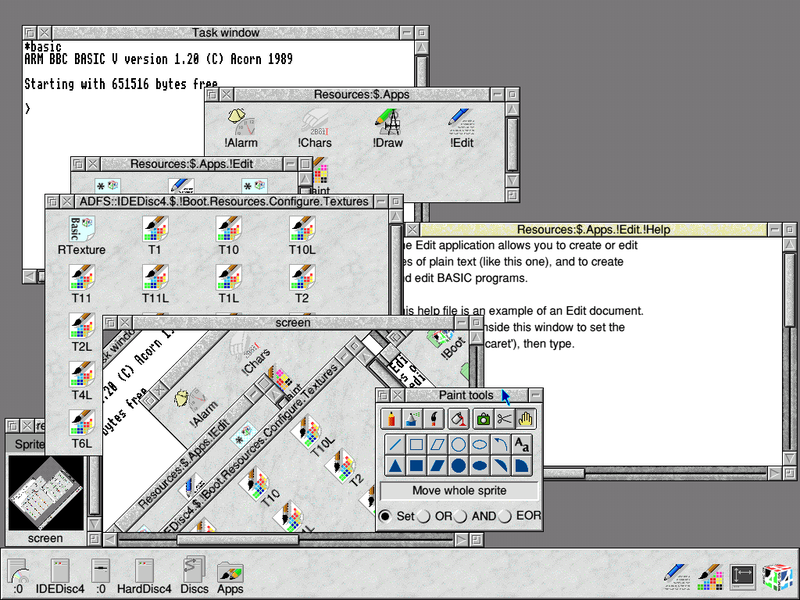
\includegraphics[width=0.8\textwidth]{figs/riscos}
\end{frame}


%----------------------------FRAME------------------------------------
\begin{frame}[fragile]\frametitle{Desde una imagen}
\begin{block}{Descargar una imagen}
\href{http://www.raspberrypi.org/downloads}{http://www.raspberrypi.org/downloads}
\end{block}

\begin{block}{Linux}
\verb|$ sudo dd if=imagen.iso of=/dev/sdc bs=1M|
\end{block}
\begin{block}{Windows}
Usar Win32DiskImager:\\
\href{http://sourceforge.net/projects/win32diskimager/}{http://sourceforge.net/projects/win32diskimager/}
\end{block}

\end{frame}


\section{Aplicaciones}

\subsection{Aplicaciones}
%----------------------------FRAME------------------------------------
\begin{frame}[fragile]\frametitle{Aplicaciones}

Ok, ya tengo una Raspberry Pi, y ahora? 
\begin{block}{Hort urbà}
\href{elmeuhort.org:2021}{elmeuhort.org:2021}

\end{block}
\begin{block}{}
\includegraphics[width=0.5\textwidth]{figs/hort}
\end{block}
\end{frame}

%----------------------------FRAME------------------------------------
\begin{frame}[fragile]\frametitle{L'Hort Unrbà}

%\flashmovie[auto=0,loop=0,controlbar=0,engine=jw-player,width=\columnwidth,heigth=\columnwidth]{video.flv}

\end{frame}

%----------------------------FRAME------------------------------------
\begin{frame}[fragile]\frametitle{Aplicaciones}

\begin{centering}
    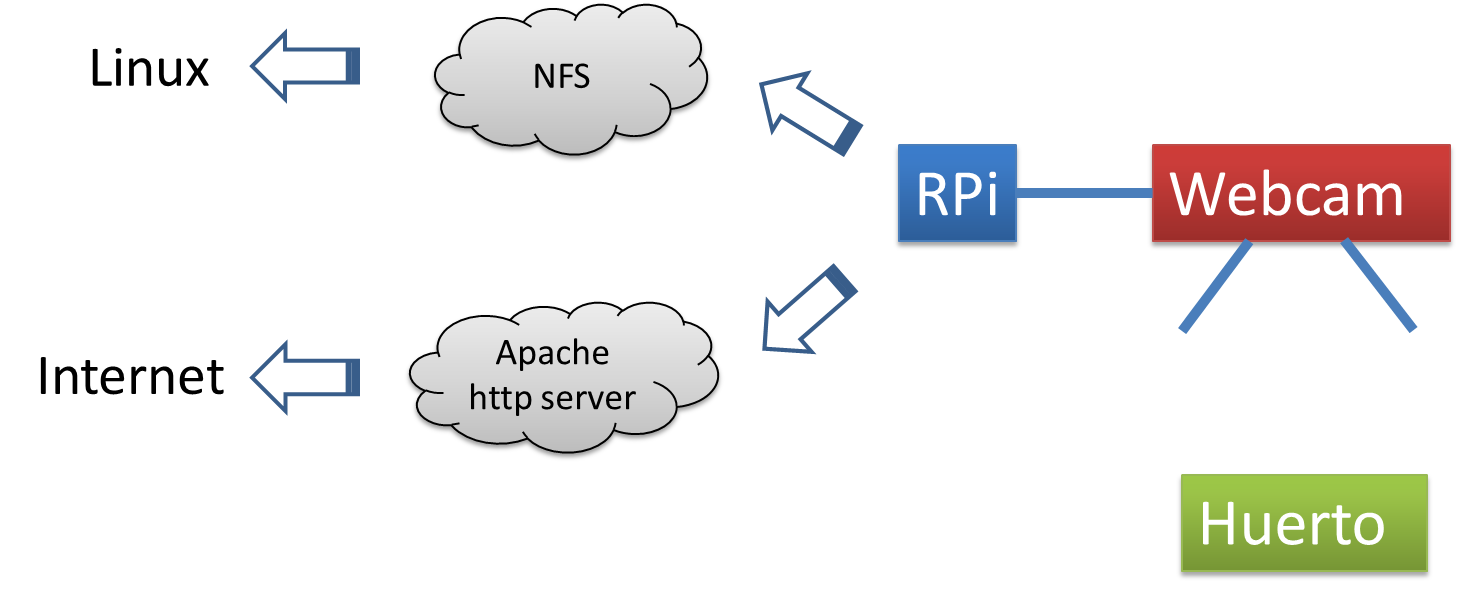
\includegraphics[width=\textwidth]{figs/short}
\end{centering}
\end{frame}


%----------------------------FRAME------------------------------------
\begin{frame}[fragile]\frametitle{xbmc}

\begin{centering}
    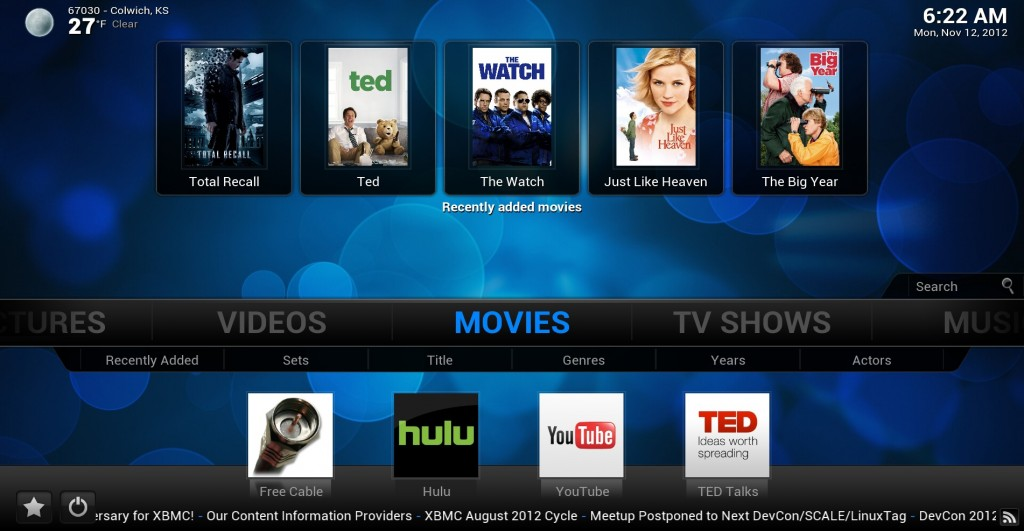
\includegraphics[width=\textwidth]{figs/xbmc}
\end{centering}


\tiny \href{http://www.elinux.org/RPi\_Projects}{http://www.elinux.org/RPi\_Projects}
\end{frame}


%----------------------------FRAME 2 cols + header (box)-------------
\begin{frame}[fragile]\frametitle{Geiger Counter}
\begin{block}{Pigi}
 \href{https://apollo.open-resource.org/lab:pigi}{https://apollo.open-resource.org/lab:pigi}
\end{block}
\begin{columns}[c]
\column{0.4\textwidth}
\begin{itemize}
    \item     A Raspberry Pi
    \item PiGI Module
    \item Geiger-Müller Tube
    \item 13 eur.
\end{itemize}
\column{0.6\textwidth}
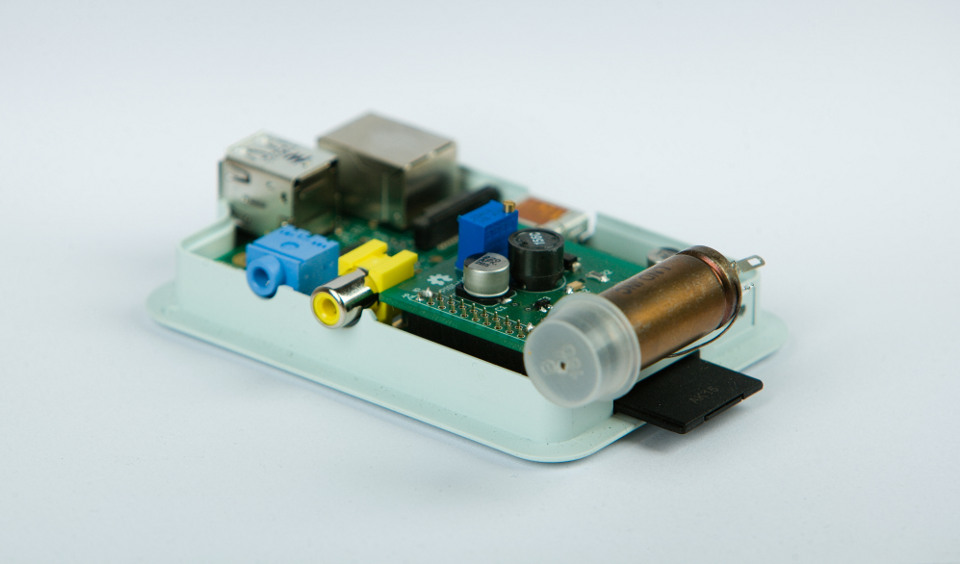
\includegraphics[width=\textwidth]{figs/geiger}
\end{columns}
\end{frame}


%----------------------------FRAME------------------------------------
\begin{frame}[fragile]\frametitle{Dropbox Clone}
\begin{block}{ownCloud}
\href{http://owncloud.org/}{http://owncloud.org/}
\end{block}
\begin{block}{BarracudaDrive}
\href{http://barracudadrive.com/RaspberryPi.lsp}{http://barracudadrive.com/RaspberryPi.lsp}
\end{block}

\end{frame}


%----------------------------FRAME------------------------------------
\begin{frame}[fragile]\frametitle{WiringPI}
\begin{block}{GPIO Interface Library for the Raspberry Pi}
\href{http://wiringpi.com}{http://wiringpi.com}
\end{block}
\begin{verbatim}
#include <wiringPi.h>
main ()
{
  wiringPiSetup () ;
  pinMode (0, OUTPUT) ;
  for (;;)
  {
    digitalWrite (0, HIGH) ; delay (500) ;
    digitalWrite (0,  LOW) ; delay (500) ;
  }
}
\end{verbatim}
\verb|gcc -Wall -o blink blink.c -lwiringPi|
\end{frame}

%----------------------------FRAME------------------------------------
\begin{frame}[fragile]\frametitle{Wiring PI}

\begin{block}{}
Wiring PI permite el acceso al GPIO en espacio de usuario.
\end{block}

\begin{minted} [bgcolor=mybg,frame=lines,bgcolor=mybg,frame=lines,bgcolor=mybg,frame=lines,mathescape]{python}
import wiringpi  
from time import sleep  
io = wiringpi.GPIO(wiringpi.GPIO.WPI_MODE_SYS)  
io.pinMode(18,io.OUTPUT)  # Setup pin 18 (GPIO1)
while True:  
    io.digitalWrite(18,io.HIGH)  # Turn on light
    sleep(2)  
    io.digitalWrite(18,io.LOW)  # Turn off
    sleep(2)

\end{minted}
\end{frame}




%----------------------------FRAME------------------------------------
\begin{frame}[fragile]\frametitle{Python blink (RPi.GPIO)}

\begin{minted} [bgcolor=mybg,frame=lines,bgcolor=mybg,frame=lines,bgcolor=mybg,frame=lines,mathescape]{python}

import RPi.GPIO as GPIO
import time
# blinking function
def blink(pin):
        GPIO.output(pin,GPIO.HIGH)
        time.sleep(1)
        GPIO.output(pin,GPIO.LOW)
        time.sleep(1)
        return
# to use Raspberry Pi board pin numbers
GPIO.setmode(GPIO.BOARD)
# set up GPIO output channel
GPIO.setup(11, GPIO.OUT)
# blink GPIO17 50 times
for i in range(0,50):
        blink(11)
GPIO.cleanup() 
\end{minted}




\end{frame}

\subsection{Gert Board}
%----------------------------FRAME------------------------------------
\begin{frame}[fragile]\frametitle{Gert Board}
\begin{block}{Espcificationes}
\begin{itemize}
    \item Acceso a los pines del GPIO de la RPi, 
    \item Acceso a los pines del ATmega.
    \item 12 digital buffers. Configurable  para entada/salida via jumpers/ 
    \item 12 LEDs conectados a los puertos digitales. 
    \item 3 botones
    \item  2 conversores canales D/A via SPI 
    \item  2 conversores canales A/D via SPI 
    \item Un controlador de motor (velocidad y dirección de un motor DC).
    \item 6 salidas en colector abierto (para relés, etc)... 
\end{itemize}
\end{block}
Fué diseñada por  Gert van Loo \href{http://www.fenlogic.com/}{http://www.fenlogic.com/}
\end{frame}

%----------------------------FRAME------------------------------------
\begin{frame}[fragile]\frametitle{Gert Board}
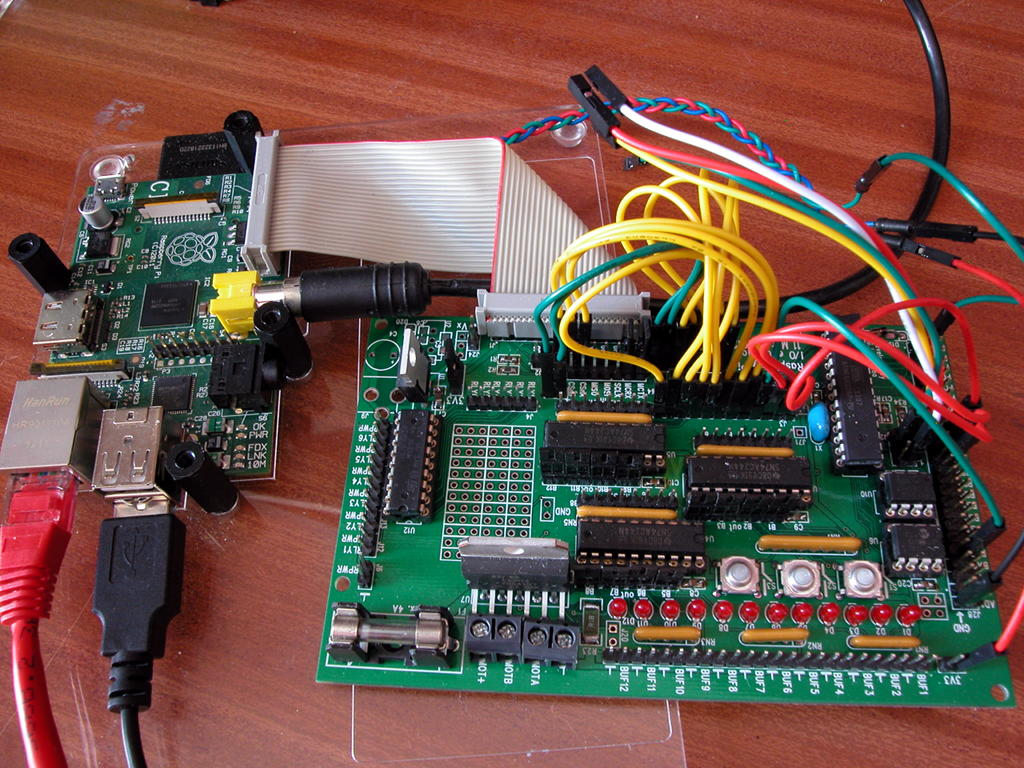
\includegraphics[width=\textwidth]{figs/gertboard1}
\end{frame}


%----------------------------FRAME------------------------------------
\begin{frame}[fragile]\frametitle{Gert Board}
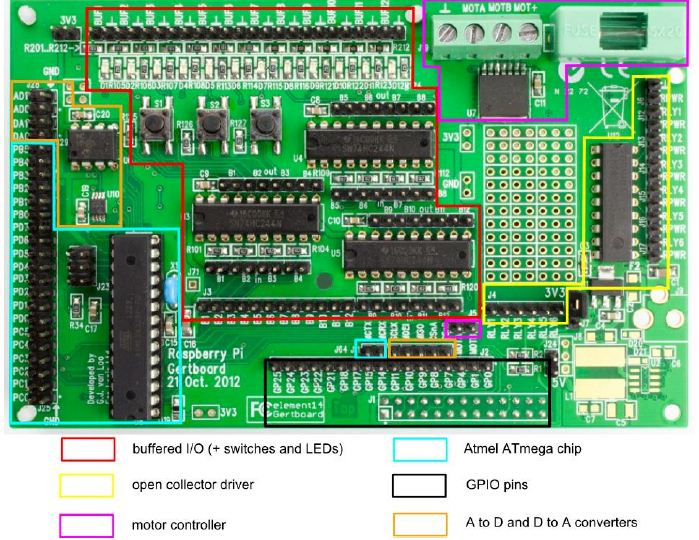
\includegraphics[width=0.85\textwidth]{figs/gertboard2}\\

\tiny \href{http://manuelaantao.blogspot.com.es/2013/03/setting-up-gertboard-io-expansion-board.html}{http://manuelaantao.blogspot.com.es/2013/03/setting-up-gertboard-io-expansion-board.html}


\end{frame}



%----------------------------FRAME------------------------------------
%\begin{frame}[fragile]\frametitle{scipi.io}
%Maybe the most common IO in SciPy is to import and export Matlab files using \emph{loadmat/savemat}. In SciPy is easy to write/read them. 
%-------------------------------CODE
%{\small
%<<label='scipy',term=True>>=
%import numpy as np
%from scipy import io as spio
%py_a = np.ones((2,2))
%spio.savemat('ex.mat',{'mat_a': py_a})
%py_mat = spio.loadmat('ex.mat')
%py_mat['mat_a']
%
%-------------------------------END CODE
%}
%where \verb|struct_as_record| loads the MATLAB structs as python objects rather than numpy structured arrays 
%\end{frame}

\section{Demo }

%----------------------------FRAME------------------------------------
\begin{frame}[fragile]\frametitle{Demo I}
\begin{center}
    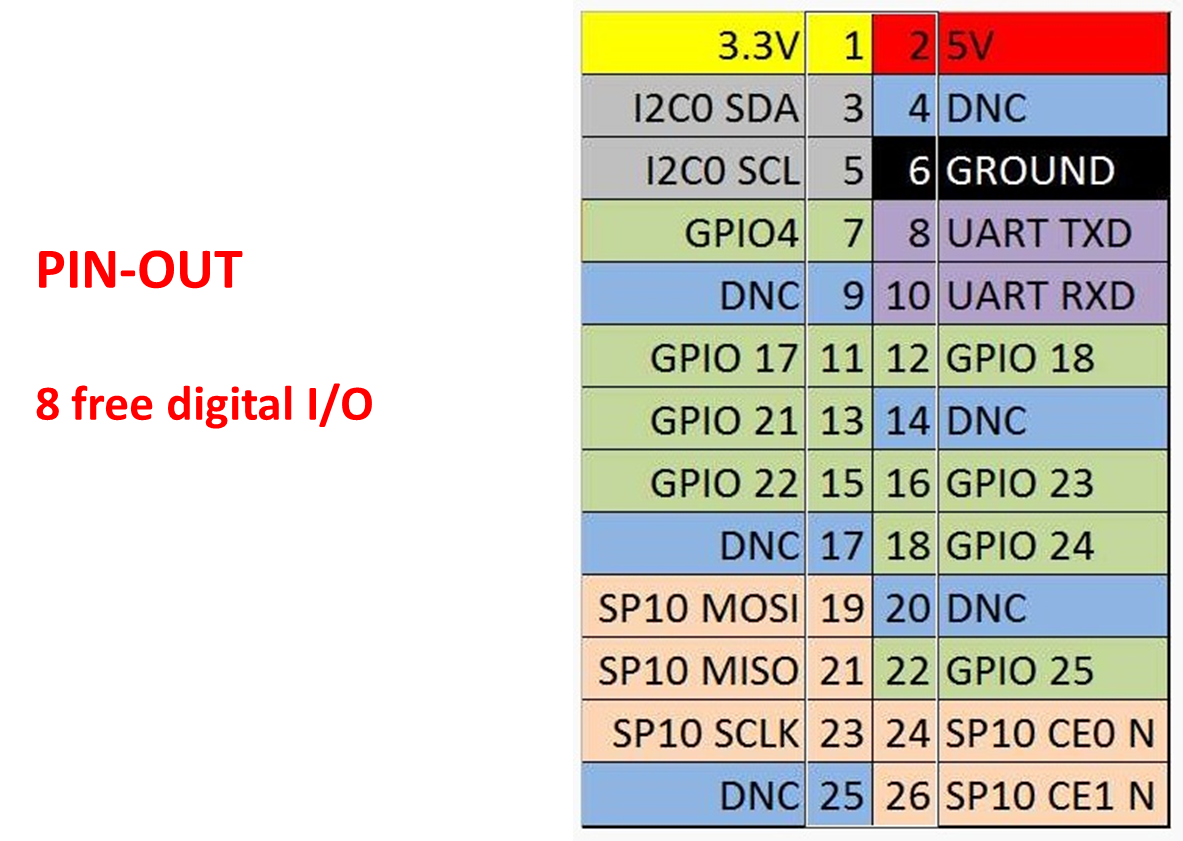
\includegraphics[width=0.8\textwidth]{figs/pin1}
\end{center}
\end{frame}


%----------------------------FRAME------------------------------------
\begin{frame}[fragile]\frametitle{Demo II}
\begin{center}
   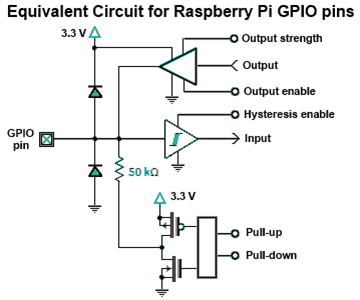
\includegraphics[width=0.8\textwidth]{figs/pin2} 
\end{center}
\end{frame}
%----------------------------FRAME------------------------------------
\begin{frame}[fragile]\frametitle{Demo II}
\begin{center}
   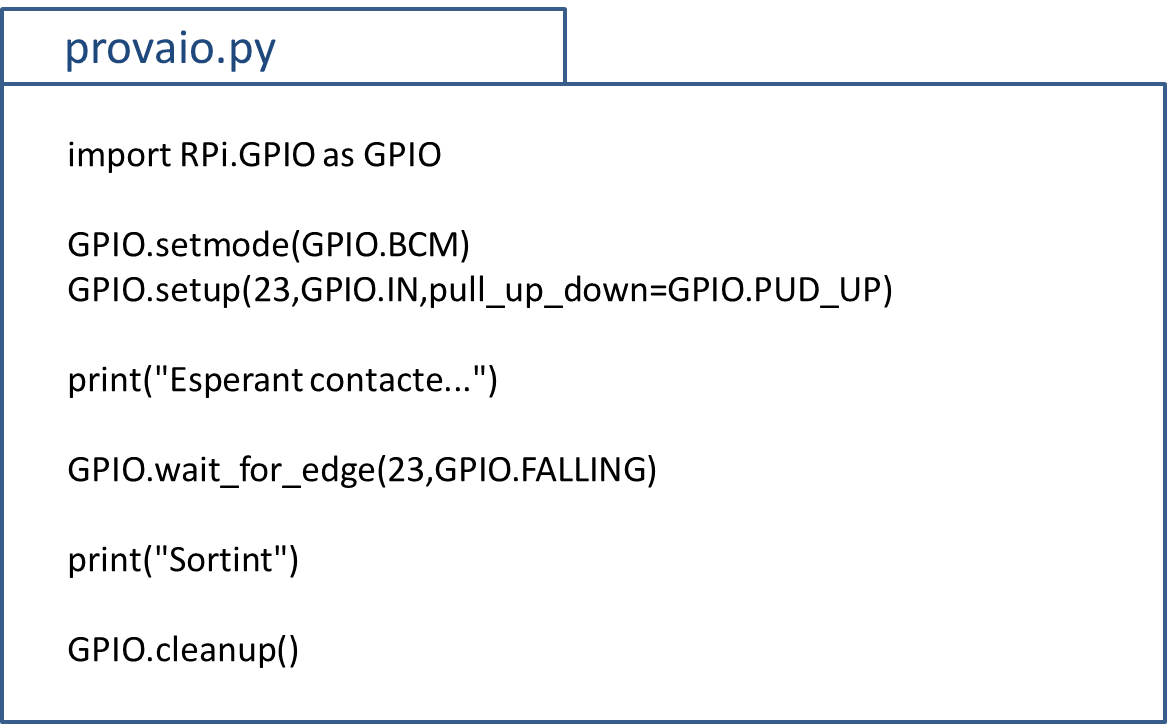
\includegraphics[width=0.8\textwidth]{figs/pin3}
\end{center}
\end{frame}

%----------------------------FRAME------------------------------------
\begin{frame}[fragile]\frametitle{Demo II}
\begin{center}
   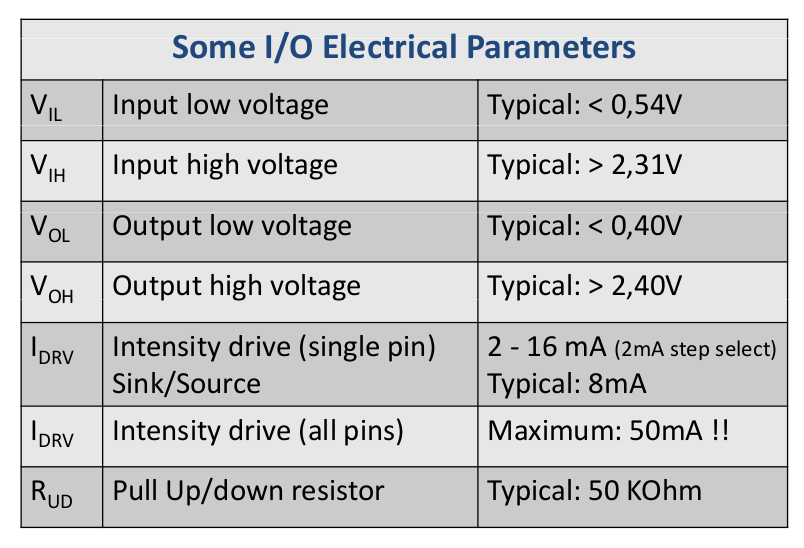
\includegraphics[width=0.8\textwidth]{figs/pin4} 
\end{center}
\end{frame}


%----------------------------FRAME------------------------------------
\begin{frame}[fragile]\frametitle{Demo IV}

\begin{verbatim}
$ sudo apt-get update
$ sudo apt-get install python-dev
$ sudo apt-get install python-rpi.gpio    
\end{verbatim}
\end{frame}



%----------------------------FRAME------------------------------------
\begin{frame}[fragile]\frametitle{Demo II}
\begin{center}
   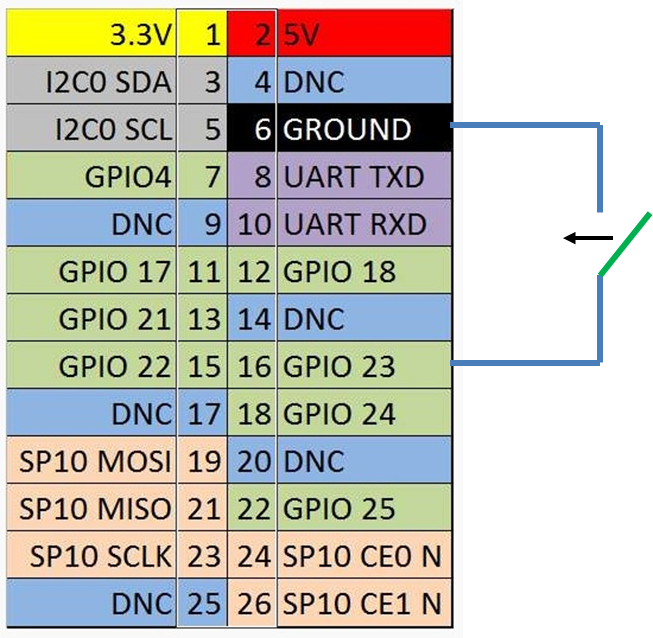
\includegraphics[width=0.8\textwidth]{figs/pin5} 
\end{center}
\end{frame}



%----------------------------FRAME------------------------------------
\begin{frame}[fragile]\frametitle{Para saber más}

\begin{itemize}
    \item \href{https://projects.drogon.net/raspberry-pi/wiringpi/}{https://projects.drogon.net/raspberry-pi/wiringpi/}
    \item \href{http://www.treehugger.com/slideshows/gadgets/20-awesome-projects-raspberry-pi-microcomputers/}{http://www.treehugger.com/slideshows/gadgets/20-awesome-projects-raspberry-pi-microcomputers/}
    \item \href{http://www.raspberrypi.org/phpBB3/}{http://www.raspberrypi.org/phpBB3/}
    \item \href{http://manuelaantao.blogspot.com.es/2013/03/setting-up-gertboard-io-expansion-board.html}{http://manuelaantao.blogspot.com.es/2013/03/setting-up-gertboard-io-expansion-board.html}
    \item \href{https://launchpad.net/win32-image-writer}{https://launchpad.net/win32-image-writer}
\end{itemize}
\end{frame}


%----------------------------FRAME------------------------------------
\begin{frame}\frametitle{Questions}
\begin{figure}[!htb]
    \centering
    
\includegraphics[width=0.6\textwidth]{figs/question_mark}
\end{figure}
\end{frame}


\end{document}
